\documentclass[a4paper,11pt]{article}
\usepackage{graphicx}
\usepackage{algorithmic}
\title{High Level Design Document \\ Bin-packing VM Consolidation Algorithm}
\author{Terli Venkatesh 13MCMT55 \\ Atchutuni Bhavana 13MCMT01 \\ Surineni Sampath Kumar 13MCMT49}
\date{}
\begin{document}
\maketitle
\pagebreak
\tableofcontents
\pagebreak

\section{Detailed Design}

\subsection{Parser Module}
This module is invoked by the GUI module to read the data from the input file given by the user and pass it to the PM-modifier.The format of the input file is specified below.\\
\begin{itemize}
\item VM\textunderscore ID---Integer
\item VM\textunderscore Capacity---Integer
\end{itemize}
\subsubsection{Interface Data Structure}
\hspace*{1.1cm}NONE
\subsubsection{Internal Data Structure}
\hspace*{1.1cm}NONE
\subsubsection{Interface Functions}
\begin{itemize}
\item int parse(filename)
\end{itemize}
\textbf{Description :}This function opens the given file.Each row in the input file should be in this format [VM\textunderscore ID, Capacity]. Parser reads each row values and calls addVM(VM\textunderscore ID,capacity) function in the PM-modifier module.\\
\\
\textbf{Input Parameters :}The path of the file given by the user from the GUI module, complete path should be specified.\\
\\
\textbf{Output Parameters :}VM\textunderscore ID,capacity.\\
\\
\textbf{Return values :} Respective error numbers will be sent for empty file and wrong file format.
\pagebreak
\\
\textbf{Pseudocode :}\\
\\
\textbf{parse(filename)}
\begin{algorithmic}[1]
\STATE open the input file which was given by GUI. 
\IF{$fp == NULL$} 
\STATE show the message you entered nonexisting filename.
\ENDIF
\STATE check whether file is empty or not.
\IF{no data in file}
\STATE show the message empty file.
\ELSE
\STATE Read the each line and send that value to addVM(VM\textunderscore ID, capacity) in PM-modifier module
\STATE this step will repeat untill we we read all the lines.
\ENDIF

\end{algorithmic}

\subsection{User Interface}
User interface is useful for taking input from  user and giving results to the user. First this module asks user to load an 
input file and passes it to parser module. After initialization of the PMs and VMs by the PM modifier module it displays a 
screen with buttons specifying the PMs and labels specifying their respective VMs.\\
It also has buttons to specify functionalities of the the system such as addVM,deleteVM and consolidate. 
\begin{figure}[h]
\centering
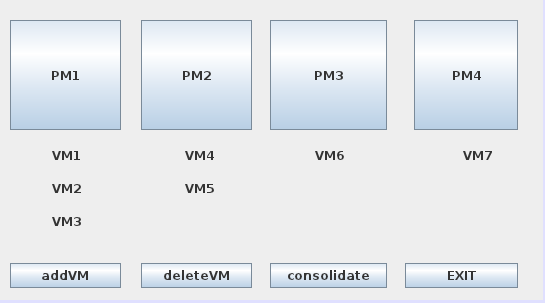
\includegraphics[height=6cm]{images/3.png}
\caption{User interface}
\end{figure}
\subsubsection{Internal Functions}
\emph{\bf callParser()}\\\\
Initially user interface has a load button.On clicking, it opens a file chooser which helps  the user to choose an input file.
\\ 
The selected input filename is passed to the parser module. \\
\begin{tabbing}
\hspace*{4cm}\= \kill
\emph{Input parameters} \>: Click event \\
\emph{Output parameters} \>: Filename \\
\emph{Returns} \>: UI is updated on success.\\ \>If the file chosen is not in the  specified format an\\ \> error message is returned.\\
\end{tabbing}
\textbf{Pseudo code :}
\begin{algorithmic}[1]
 \STATE on clicking load
 \STATE open file chooser
  \IF {file choosen}
  \STATE call parser(filename) in parser module
  \STATE call updateUI()
  \ELSE 
  \STATE no change
  \ENDIF
 \end{algorithmic}
\begin{figure}[ht!]
\centering
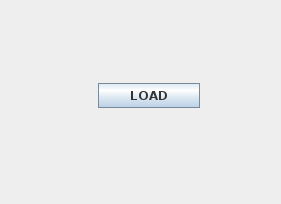
\includegraphics[height=5cm]{images/1.png}
\caption{Initial GUI}
\end{figure}
\begin{figure}[h]
\centering
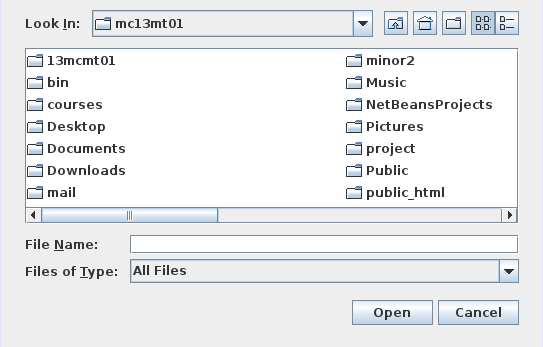
\includegraphics[height=6cm]{images/2.png}
\caption{File chooser}
\end{figure}
\begin{figure}[h]
 \centering
 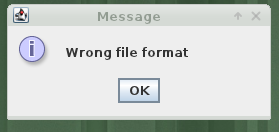
\includegraphics[height=3cm]{images/7.png}
 \caption{Error message}
\end{figure}
\pagebreak
\mbox{}\\\\
\emph{\bf callAddVM()}\\\\
 On click addVM button,a dialog asking the user to enter VM\textunderscore ID and  capacity opens.
  Once the user specifies VM\textunderscore ID and its capacity it calls the addVM() in PM modifier module and then calls updateUI().
  \\
  \begin{figure}[ht!]
 \centering
 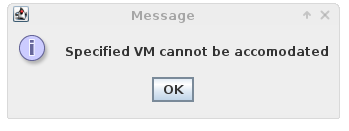
\includegraphics[scale=0.5, angle=0]{images/8.png}
 \caption{Error message}
\end{figure}
\pagebreak
\\
  \begin{tabbing}
  \hspace*{4cm}\= \kill
  \emph{Input parameters}\>: Click event\\
\emph{Output parameters}\>: VM\textunderscore ID, capacity\\
\emph{Returns}\>: UI is updated on success. \\ \> Error message is returned if the specified VM cannot be \\ \> accommodated by any of the PMs.\\
\emph{Error condition} \>: Entering negative numbers,alphanumerics,special \\ \> characters, numbers greater than  physical machine \\ \>capacity can be avoided by data validation.
 \\
 \end{tabbing}
  \textbf{Pseudo code :}
 \begin{algorithmic}[1]
\STATE on clicking addVM
\STATE open dialog asking for VM\textunderscore ID and capacity
\STATE validate input
\IF {valid}
\STATE call addVM(VM\textunderscore ID,capacity) in PM modifier
\STATE call updateUI()
\ELSE 
\STATE show error message
\ENDIF
 \end{algorithmic}
\mbox{}\\\\
 \emph{\bf callDeleteVM()}\\\\
 On clicking the deleteVM button in user interface, it opens a dialog  which prompts the user to choose a VM for deletion.
 This calls the deleteVM() in PM modifier module. Later calls updateUI().
 \\  \begin{tabbing}
   \hspace*{4cm}\= \kill
 
 \emph{Input parameters}\>: Click event\\
 \emph{Output parameter}\>: VM\textunderscore ID\\
\emph{Returns}\>: UI is updated on success.\\
\emph{Error conditions}\>: Choosing an incorrect VM\textunderscore ID. But this case is avoided \\ \> by listing all the VMs present in the system.
\end{tabbing}
\begin{algorithmic}[1]
 \STATE on clicking deleteVM
 \STATE open dialog displaying list of VMs, asking user to choose VM for deletion
 \IF {choosen}
 \STATE call deleteVM(VM\textunderscore ID)
 \STATE call updateUI()
 \ELSE
 \STATE do nothing
 \ENDIF
 \end{algorithmic}
\begin{figure}[ht!]
\centering
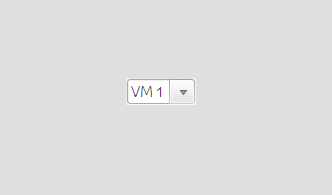
\includegraphics[scale=0.8, angle=0]{images/4.png}
\caption{VM Deletion}
\end{figure}
\mbox{}\\\\
\emph{\bf callConsolidate()}\\\\
On clicking consolidate button in UI it opens a dialog for confirmation from the user \\
If the user chooses not to consolidate the state of the system does not change.\\
If the user chooses to consolidate ,  then conolidate() funtion in PM modifier is called.
\\ The user interface is updated using the updateUI() function.
\\
  \begin{tabbing}
  \hspace*{4cm}\= \kill
\emph{Input parameters}\>: Click event
\\
\emph{Output parameters}\>: None \\
\emph{Returns}\>: UI is updated and the color of the physical machines\\ \> that are switched off changes.\\
\emph{Error condition} \>: None\\
\end{tabbing}
\textbf{Pseudo code :}
\begin{algorithmic}[1]
\STATE on clicking consolidate
\STATE open dialog for confirmation
\IF {confirmed}
\STATE call consolidate()
\STATE call updateUI()
\ELSE 
\STATE do nothing
\ENDIF
\end{algorithmic}
\begin{figure}[ht!]
\centering
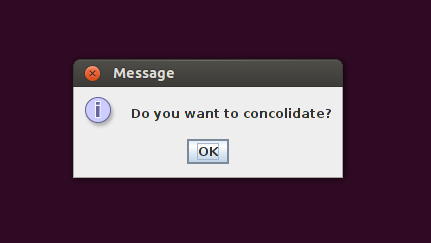
\includegraphics[scale=0.6, angle=0]{images/5.png}
\caption{Consolidation}
\end{figure} 
\mbox{}\\\\
\emph{\bf updateUI()}\\\\
This function is called after every change performed on the system to reflect changes to the user.It calls the status() function in PM modifier module.
\\\begin{tabbing}
  \hspace*{4cm}\= \kill

\emph{Input parameters}\>: None
\\
\emph{Output parameters}\>: None\\
\emph{Returns}\>: Updated UI\\
\emph{Error conditions}\>: None\\
\end{tabbing}
\textbf{Pseudo code :}
\begin{algorithmic}[1]
 \STATE call status()
 \STATE accordingly modify PMs and VMs
\end{algorithmic}
\mbox{}\\\\
\emph{\bf onPM()}\\\\
This function is used to switch on a PM manually by the user.When user clicks a PM  which is in off state,changes its state to ON by calling the switchOnPM() function in PM modifier.Then calls updateUI().
If user chooses a PM that is already in on state ,a message is prompted to user if he/she wishes to turn off respective PM
\\\begin{tabbing}
  \hspace*{4cm}\= \kill
\emph{Input parameters}\>: Click event\\
\emph{Output parameters}\>: PM\textunderscore ID\\
\emph{Returns}\>: UI is updated on success.The color of the PM that is \\ \> turned on changes.On failure returns an error message.\\ 
\end{tabbing}
\textbf{Pseudo code :}
\begin{algorithmic}[1]
 \STATE on clicking PM 
 \IF {PM in OFF state}
 \STATE OPEN DIALOG FOR CONFIRMATION
 \IF {confirmed}
 \STATE call switchOnPM() in PM modifier
 \ELSE 
 \STATE no change
 \ENDIF
 \ENDIF
\end{algorithmic}
\mbox{}\\\\
\emph{\bf offPM()}
\\\\
This function is used to switch off a PM manually by the user.When user clicks a PM which is turned on,changes its state to OFF by calling switchOffPM() function in PM modifier.
\\\begin{tabbing}
  \hspace*{4cm}\= \kill
  \emph{Input parameters}\>: Click event\\
  \emph{Output parameters}\>: PM\textunderscore ID\\
  \emph{Returns}\>: UI is updated on success.The color of the PM that is \\ \> turned off changes.On failure returns an error message.\\
  \emph{Error conditions}\>: If the VMs in selected PM cannot be accommodated in another PMs.
  \end{tabbing}
  \textbf{Pseudo code :}
  \begin{algorithmic}[1]
   \STATE on clicking PM 
   \IF {PM is in ON state}
   \STATE open dialog for confirmation
   \IF {confirmed}
   \STATE call switchOffPM()
   \IF {no error}
   \STATE call updateUI()
   \ELSE 
   \STATE show error message
   \ENDIF
   \ELSE
   \STATE no change
   \ENDIF
   \ENDIF
  \end{algorithmic}
\pagebreak
\subsection{PM Modifier Module}
This module will be called by Parser module and User Interface module for
\begin{itemize}
 \item Adding a Virtual Machine(VM),
 \item Deleting a VM,
 \item Switching off a PM,
 \item Switching on a PM and
 \item Consolidation
\end{itemize}
\subsubsection{Interface Data Structures}
\begin{enumerate}
 \item PMstruct
 \end{enumerate}
\textbf{PMstruct}
\\

Different fields in PMstruct data structure are
\begin{enumerate}
 \item PM\textunderscore ID - final String
 \item res\textunderscore cap - integer
 \item VM\textunderscore list - array of type class VMstruct
 \item onSate - integer
\end{enumerate}

This is the data structure returned to status() function which is called by User Interface
\\
\subsubsection{Internal Data Structures}
\begin{enumerate}
 \item VMstruct
\end{enumerate}
\textbf{VMstruct}
\\

Different fields in VMstruct data structure are
\begin{enumerate}
 \item VM\textunderscore ID - final String
 \item cap - integer
\end{enumerate}
This is the structure used by PM modifier to create a VM.
\subsubsection{Interface Functions}
\textbf{void addVM(VM\textunderscore ID, cap)}
\\
\textbf{Description :} This function checks the PM's if there is enough capacity available and if available adds the VM to it. If there is no enough capacity 
it returns an error.
\\
\textbf{Input parameters :} The cap of VM which is to be added. The ID for VM is automatically generated by the function.
\\
\textbf{Output parameters :} NONE.
\\
\textbf{Return Values :} If sufficient capacity to add a VM is not available it returns \textbf{No enough capacity} error message
\\
\textbf{Pseudocode :}
\begin{algorithmic}[1]
\STATE void addVM(\emph{VM\textunderscore ID, cap)}
\FOR {\textbf{each} \emph{PMstruct} \textbf{in} \emph{PMlist}}
\IF {\emph{res\textunderscore cap} $\leq 1$ \emph{cap}}
\STATE create an ID for this VM
\STATE add VM to this PM
\ENDIF
\ENDFOR
\end{algorithmic}
\mbox{}\\\\
\textbf{void deleteVM(VM\textunderscore ID)}
\\
\textbf{Description :} The purpose of this function is to delete the VM which is passed as an input parameter to while calling this function.
\\
\textbf{Input parameters :} The VM\textunderscore ID of VM which has to be deleted.
\\
\textbf{Output parameters :} NONE.
\\
\textbf{Return Values :} None, because all the error conditions that may arise are handled by data validation in user interface.
\\
\textbf{Pseudocode :}
\begin{algorithmic}[1]
\STATE void deleteVM(\emph{VM\textunderscore ID)}
\FOR {\textbf{each} \emph{PMstruct} \textbf{in} \emph{PMlist}}
\FOR {\textbf{each} \emph{VMstruct} \textbf{in} \emph{VMarray}}
\IF {\emph{VM\textunderscore ID} matches}
\STATE delete this VM
\ENDIF
\ENDFOR
\ENDFOR
\end{algorithmic}
\mbox{}\\\\
\pagebreak
\\
\textbf{ void switchOffPM(PM\textunderscore ID)}
\\
\textbf{Description :} This function switches off the specified PM.
\\
\textbf{Input parameters :} PM ID of the PM which has to be switched off.
\\
\textbf{Output parameters :} NONE.
\\
\textbf{Return Values :} Returns error if the VM's in the current PM can't be consolidated in to other PM's.
\\
\textbf{Pseudocode :}
\begin{algorithmic}[1]
\STATE void switchOffPM(\emph{PM\textunderscore ID})
\FOR {\textbf{each} \emph{PMstruct} \textbf{in} \emph{PMlist}}
\IF {\emph{PM\textunderscore ID} matches}
\STATE change onState to OFF
\ENDIF
\ENDFOR
\end{algorithmic}
\mbox{}\\\\
\textbf{ void switchOnPM(PM\textunderscore ID)}
\\
\textbf{Description :} This function switches on the specified PM.
\\
\textbf{Input parameters :} PM ID of the PM which has to be switched on.
\\
\textbf{Output parameters :} NONE.
\\
\textbf{Return Values :} No possible error condition.
\\
\textbf{Pseudocode :}
\begin{algorithmic}[1]
\STATE void switchOnPM(\emph{PM\textunderscore ID})
\FOR {\textbf{each} \emph{PMstruct} \textbf{in} \emph{PMlist}}
\IF {\emph{PM\textunderscore ID} matches}
\STATE change onState to ON
\ENDIF
\ENDFOR
\end{algorithmic}
\mbox{}\\\\
\textbf{ void consolidate()}
\\
\textbf{Description :} The function runs the consolidation algorithm to consolidate VM's in PM's and swithces 
off the PM's if any of the PM's become empty after consolidation.
\\
\textbf{Input parameters :} NONE.
\\
\textbf{Output parameters :} NONE.
\\
\textbf{Return Values :} No possible error conditions
\\
\textbf{Pseudocode :}
\begin{algorithmic}[1]
\STATE void consolidate()
\STATE quicksort(\emph{PMlist,lo,hi}) \COMMENT{sorts PMs in decreasing order of their residual capacity}
\FOR {\emph{i} from \emph{0} to \emph{PMlist.lenght-1}}
\STATE quicksort(\emph{PMlist[i].VMarray, lo, hi}) \COMMENT{sorts VMs in decreasing order of their capacity}
\FOR {\textbf{each} \emph{VMstruct} \textbf{in} \emph{VMarray}}
\FOR {\emph{i} from \emph{PMlist.lenght-1} to \emph{0}}
\IF {\emph{PMlist[i].PMstruct.res\textunderscore cap} $ \geq $\emph{VMarray.VMstruct.cap}}
\STATE move VMstruct into this PMstruct's VMarray
\ENDIF
\ENDFOR
\ENDFOR
\ENDFOR
\end{algorithmic}
\mbox{}\\\\
Method used to sort PM's and VM's.
\begin{algorithmic}[1]
\STATE void \textbf{quicksort}(\emph{PMlist,lo,hi})
\IF {\emph{lo} $ < $ \emph{hi}}
\STATE p = pivot(\emph{PMlist,lo,hi})
\STATE left, right = partition(\emph{PMlist, p, lo, hi})
\STATE quicksort(\emph{PMlist, lo, left})
\STATE quicksort(\emph{PMlist, right, hi})
\ENDIF
\end{algorithmic}
\mbox{}\\\\
\begin{algorithmic}[1]
\STATE int \textbf{partition}(\emph{PMlist, left, right, pivotIndex})
\STATE pivotValue = PMlist[pivotIndex]
\STATE swap PMlist[pivotIndex] and PMlist[right]
\STATE storeIndex = left
\FOR {\emph{i} from \emph{left} to \emph{right - 1}}
\IF {\emph{PMlist[i]} $\leq 1$ \emph{pivotValue}}
\STATE swap \emph{PMlist[i]} and \emph{PMlist[storeIndex]}
\STATE \emph{storeIndex} = \emph{storeIndex} + 1
\ENDIF
\STATE swap \emph{PMlist[storeIndex]} and \emph{PMlist[right]}
\ENDFOR
\RETURN \emph{storeIndex}
\end{algorithmic}
\end{document}
